
\begin{comment}
\begin{figure*}
    \centering   
		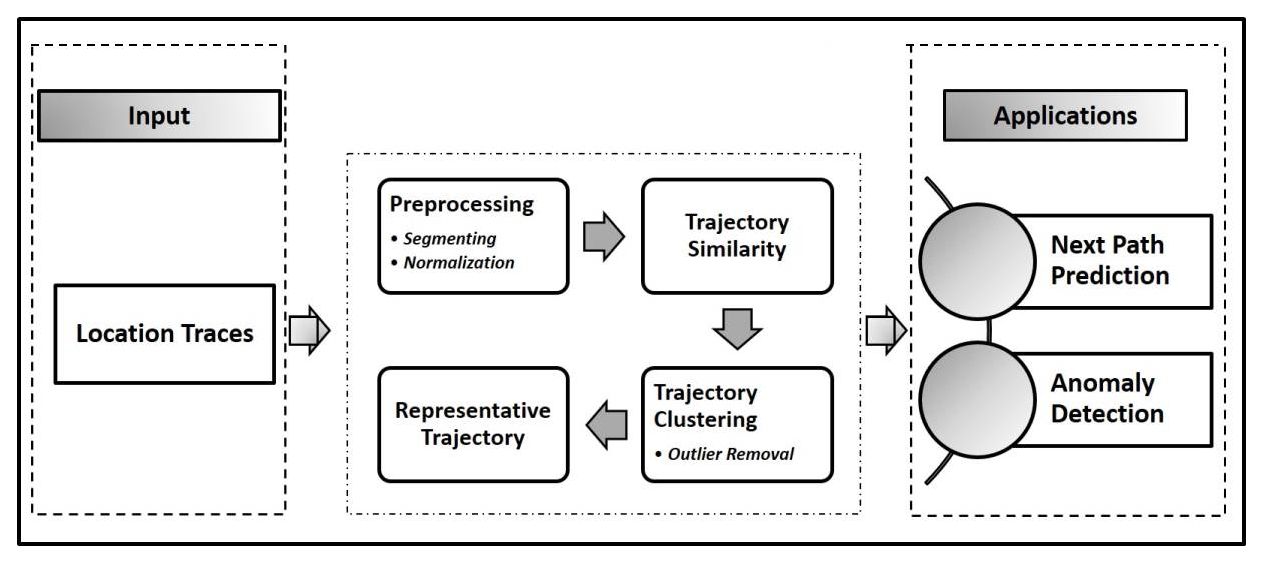
\includegraphics[scale=0.5]{figs/system_arch.eps}
		\caption{Visualization Framework.}
		\label{fig:vis}  
\end{figure*}
\end{comment}


\paragraph{Visualization}
\label{sec:vis}
Fig. \ref{fig:vis} shows a screen-shot of the visualization framework which has been created to work with the trajectories, and the summaries of the user. The interactive framework shows the mobility summary different users. The tool allows exploration of clusters formed at various zoom levels of space. With this flexibility, the tool allows choosing arbitrary level of abstraction of movement summary (e.g., at a city level or at a more granular trajectory level). 
%Once the number of clusters( say k) is set, the k clusters formed will be shown, each cluster in a different colour. 
The tool shows the representative trajectory of each cluster; the thickness is proportional to the number of trajectories in the cluster. Further, each cluster can be individually chosen and inspected. 